\documentclass{beamer}
 
\usepackage[utf8]{inputenc}
\usepackage{374_preamble}
\newcommand{\ta}[1]{\text{#1}}
\usepackage{qtree}
\usepackage{soul}
\usepackage{graphicx}
\usepackage{outlines}
\usepackage{array}
\usepackage{bm}
\graphicspath{./pictures}
 
 
%Information to be included in the title page:
\title{Senior Thesis Progress}
 
 
 
\begin{document}

 
\frame{\titlepage}


\begin{frame}
    \frametitle{Outline}
    \begin{outline}
        \1<1-> Problem Statement
        \2<2-> Background of Phenomena and Technologies
        \2<2-> Detailed Problem Statement
        \1<3-> Current Progress
        \2<4-> Month by month breakdown.
        \2<4-> Position with respect to milestones
        \1<5-> Remaining Work
        \2<6-> Technical Details
        \2<6-> Execution Plan
    \end{outline}
\end{frame} 

\begin{frame}
    \frametitle{Problem Statement}
    \begin{block}{TLDR}
        Make a dishwasher autonomously turn on when electricity is
        cheapest.
    \end{block}
\end{frame}

%After slide 1, tangent to discuss a Particle Photon
\begin{frame}
    \frametitle{Background}
    \begin{block}{IOT}
        Intelligently interact with everyday objects over a network.
    \end{block}
\end{frame}

\begin{frame}
    \frametitle{Particle}
    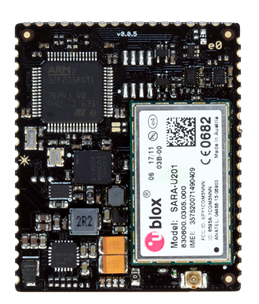
\includegraphics[width=0.6\paperwidth,height=0.6\paperheight,keepaspectratio]{pictures/particle}
\end{frame}

%After slide 2, tangent to discuss Serverless Computing.
\begin{frame}
    \frametitle{Background}
    \begin{block}{IOT}<1->
        Intelligently interact with everyday objects over a network.
    \end{block}
    \begin{block}{Serverless Computing}<2->
        Outsource the maintenance of a server to a third party. Focus on the product. 
    \end{block}
\end{frame}

\begin{frame}
    \begin{block}{Example of Serverless Computing}
        \begin{outline}
            \1 <1-> Kellog's spends 1/3 of its revenue on trade spend.
            \2 <2-> Optimize trade spend over choices:
            \3 <2-> Coupons
            \3 <2-> Ad campaigns
            \3 <2-> TV ad spend
            \3 <2-> Shelving and Display
            \1 <3-> Until 2013, Kellog's ran queries on an on-premise, relational
            database.
            \1 <4-> Reached 16 TB data
            \2 <5-> They outsourced the infrastructure needed to run and store 
            these queries to AWS (Amazon Web Services).
        \end{outline}
    \end{block}
\end{frame}

%Return to Background in order to introduce Electricity Price Variability.
\begin{frame}
    \frametitle{Background}
    \begin{block}{IOT}<1->
        Intelligently interact with everyday objects over a network.
    \end{block}
    \begin{block}{Serverless Computing}<1->
        Outsource the maintenance of a server to a third party. Focus on the product. 
    \end{block}
    \begin{block}{Electricity Price Variability}<2->
        Predict when rates are the cheapest. 
    \end{block}
\end{frame}

\begin{frame}
    \frametitle{Price Data from ComEd in Illinois}
    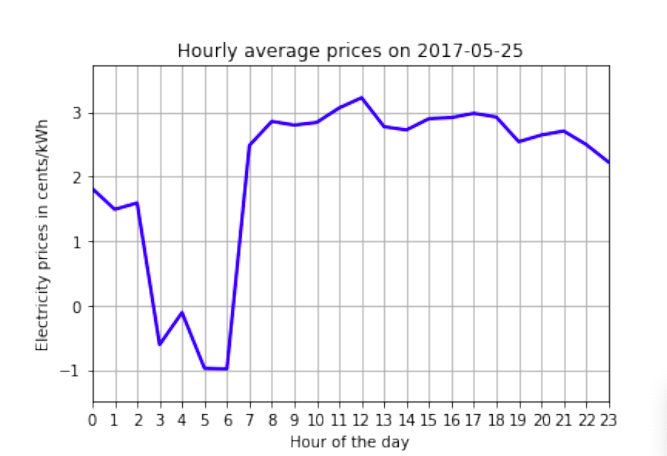
\includegraphics[width=0.9\paperwidth,height=0.8\paperheight,keepaspectratio]{pictures/average_hourly_prices}
    \cite{Jemand2000} 
\end{frame}

\begin{frame}
    \frametitle{Background}
    \begin{block}{IOT}<1->
        Intelligently interact with everyday objects over a network.
    \end{block}
    \begin{block}{Serverless Computing}<1->
        Outsource the maintenance of a server to a third party. Focus on the product. 
    \end{block}
    \begin{block}{Electricity Price Variability}<1->
        Predict when rates are the cheapest. \cite{Sowers2017}
    \end{block}
    \begin{block}{Environmental Appeal}<2->
        There is high correlation between prices are cheap and low grid demand,
        which is in turn correlated with more environmentally
        friendly uses of power \cite{Mooney2015} \cite{Lombard2008}.
    \end{block}
\end{frame}

%Now give the full research problem:
\begin{frame}
    \frametitle{Full Problem}
    \begin{outline}
        \1<1-> Frame a heuristic in place of identifying when electricity prices are cheapest.
        \1<2-> Make an algorithm to solve that heuristic.
    \end{outline}
\end{frame}

\begin{frame}
    \frametitle{Algorithm}
    \begin{outline}
        \1<1-> Run the algorithm every hour from 12AM to 5AM until the algorithm says ``yes.''
        \1<2-> Classify between 3AM and 4AM.
    \end{outline}
\end{frame}

\begin{frame}
    \frametitle{Full Problem}
    \begin{outline}
        \1<1-> Frame a heuristic in place of identifying when electricity prices are cheapest.
        \1<1-> Make an algorithm to solve that heuristic.
        \1<2-> Make a subscription service that allows consumers to enable their electricity
        appliances to turn on at later, cheaper times.
    \end{outline}
\end{frame}

\begin{frame}
    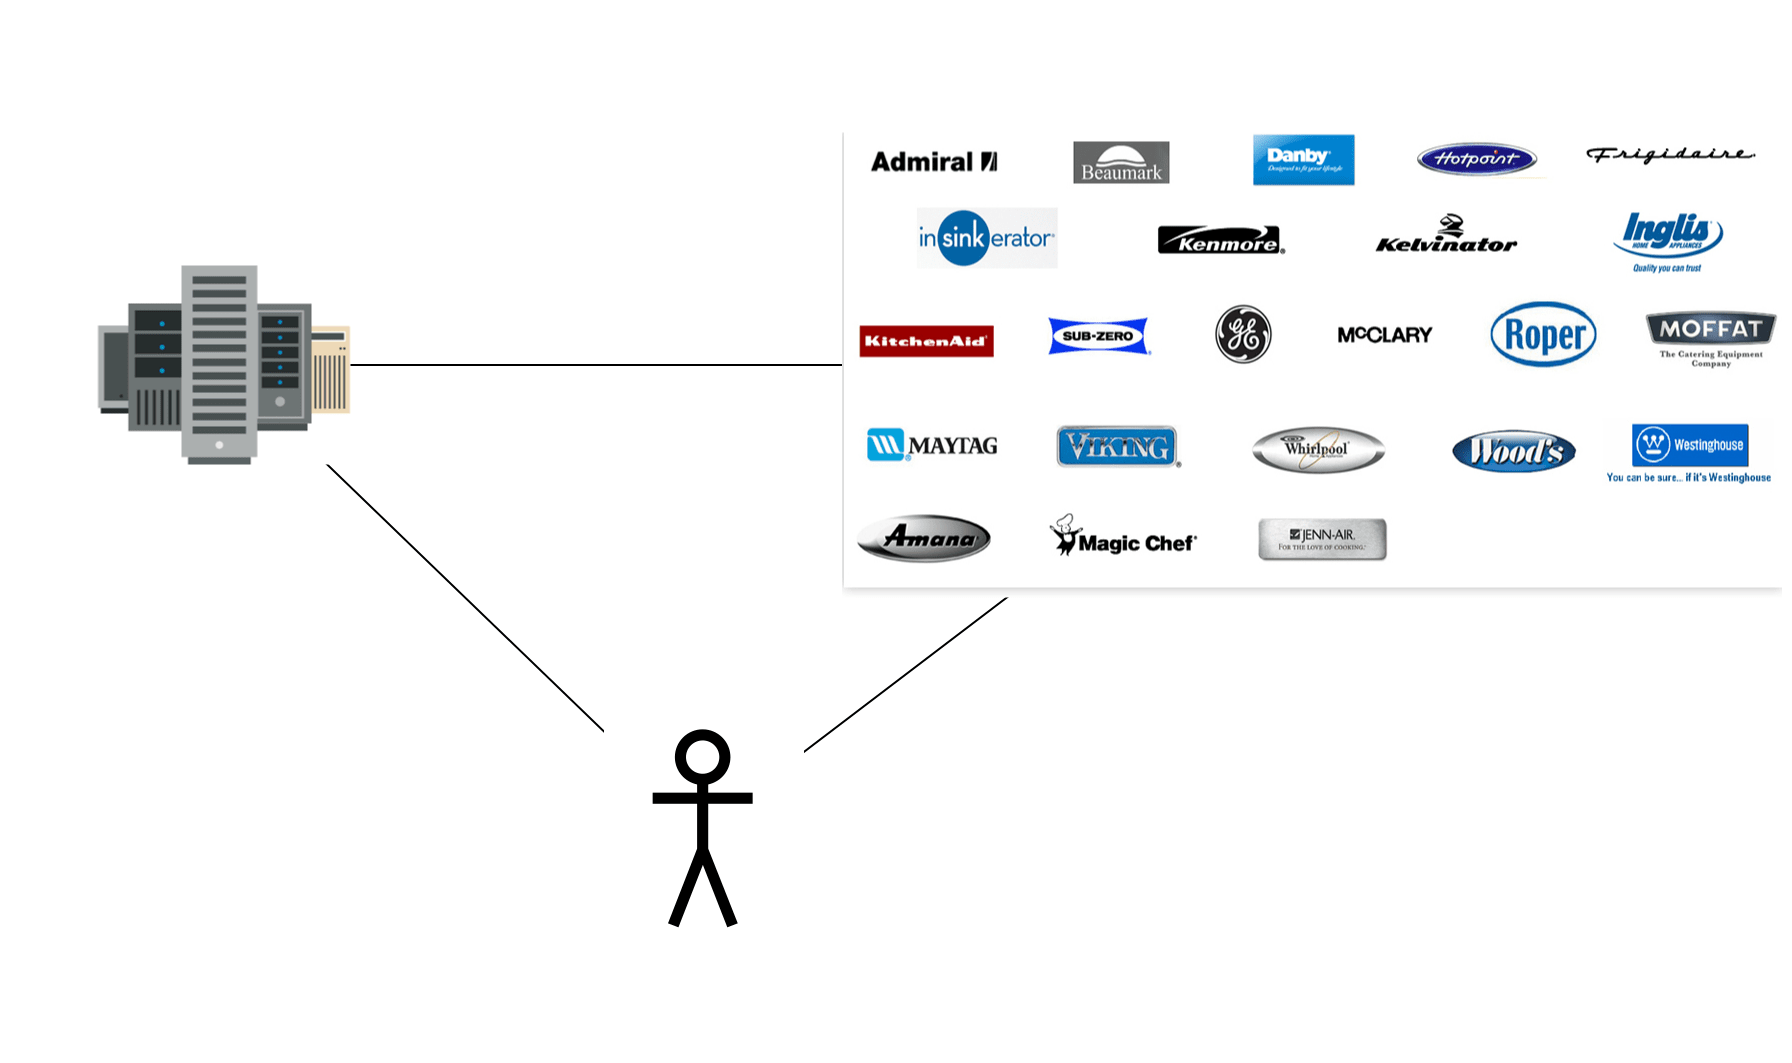
\includegraphics[width=0.9\paperwidth,height=0.8\paperheight,keepaspectratio]{pictures/service_model}
\end{frame}

\begin{frame}
    \frametitle{Full Problem}
    \begin{outline}
        \1<1-> Frame a heuristic in place of identifying when electricity prices are cheapest.
        \1<1-> Make an algorithm to solve that heuristic.
        \1<1-> Make a subscription service that allows consumers to enable their electricity
        appliances to turn on at later, cheaper times.
        \2<2-> Does this service scale well when used with many clients? What are the
        results from a heavy simulation?
        \2<3-> Does this service actually save money when physically implemented \cite{Faruqui2010}? Can we, as service providers, make the service profitable?
        \2<4-> If time permits: If such a service begins to be used en masse, what
        outlook does the profitability of it have? Is there still a profit that can be made?
    \end{outline}
\end{frame}

\begin{frame}
    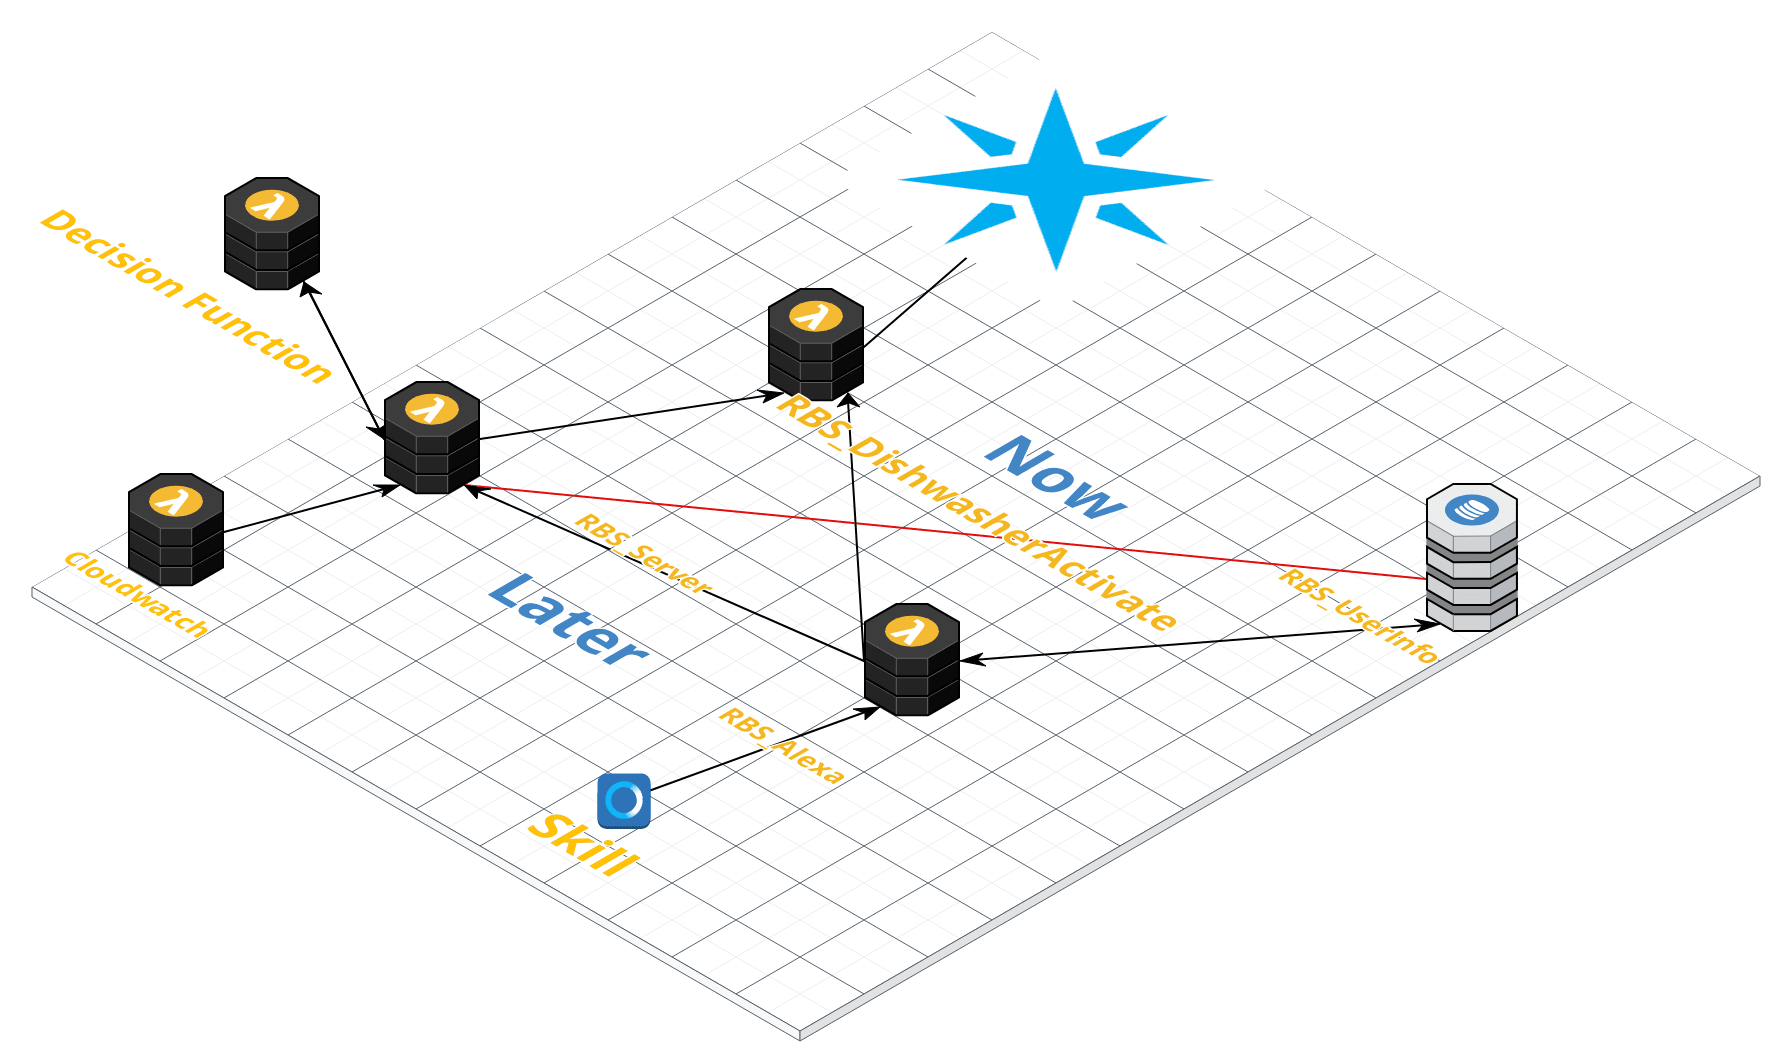
\includegraphics[width=\paperwidth,height=\paperheight,keepaspectratio]{pictures/architecture}
\end{frame}

\begin{frame}
    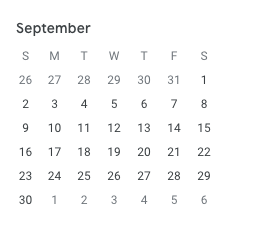
\includegraphics[width=0.5\paperwidth,height=0.5\paperheight,keepaspectratio]{pictures/september}

    \begin{outline}
        \1<1-> Learned how to work with:
        \2<2-> AWS
        \3<2-> Lambda
        \3<2-> DynamoDB
        \3<2-> Cloudwatch
        \2<3-> Javascript and Node
        \2<4-> Particle
    \end{outline}
\end{frame}

\begin{frame}
    
\includegraphics[width=0.5\paperwidth,height=0.5\paperheight,keepaspectratio]{pictures/october}
    \begin{outline}
        \1<1-> First two weeks:
        \2<1-> Revived Old Infrastructure
        \1<2-> Second two weeks:
        \2<2-> Scaled the existing infrastructure to work with two appliances for one user
        when invoking the appliance immediately.
    \end{outline}
\end{frame}

\begin{frame}
    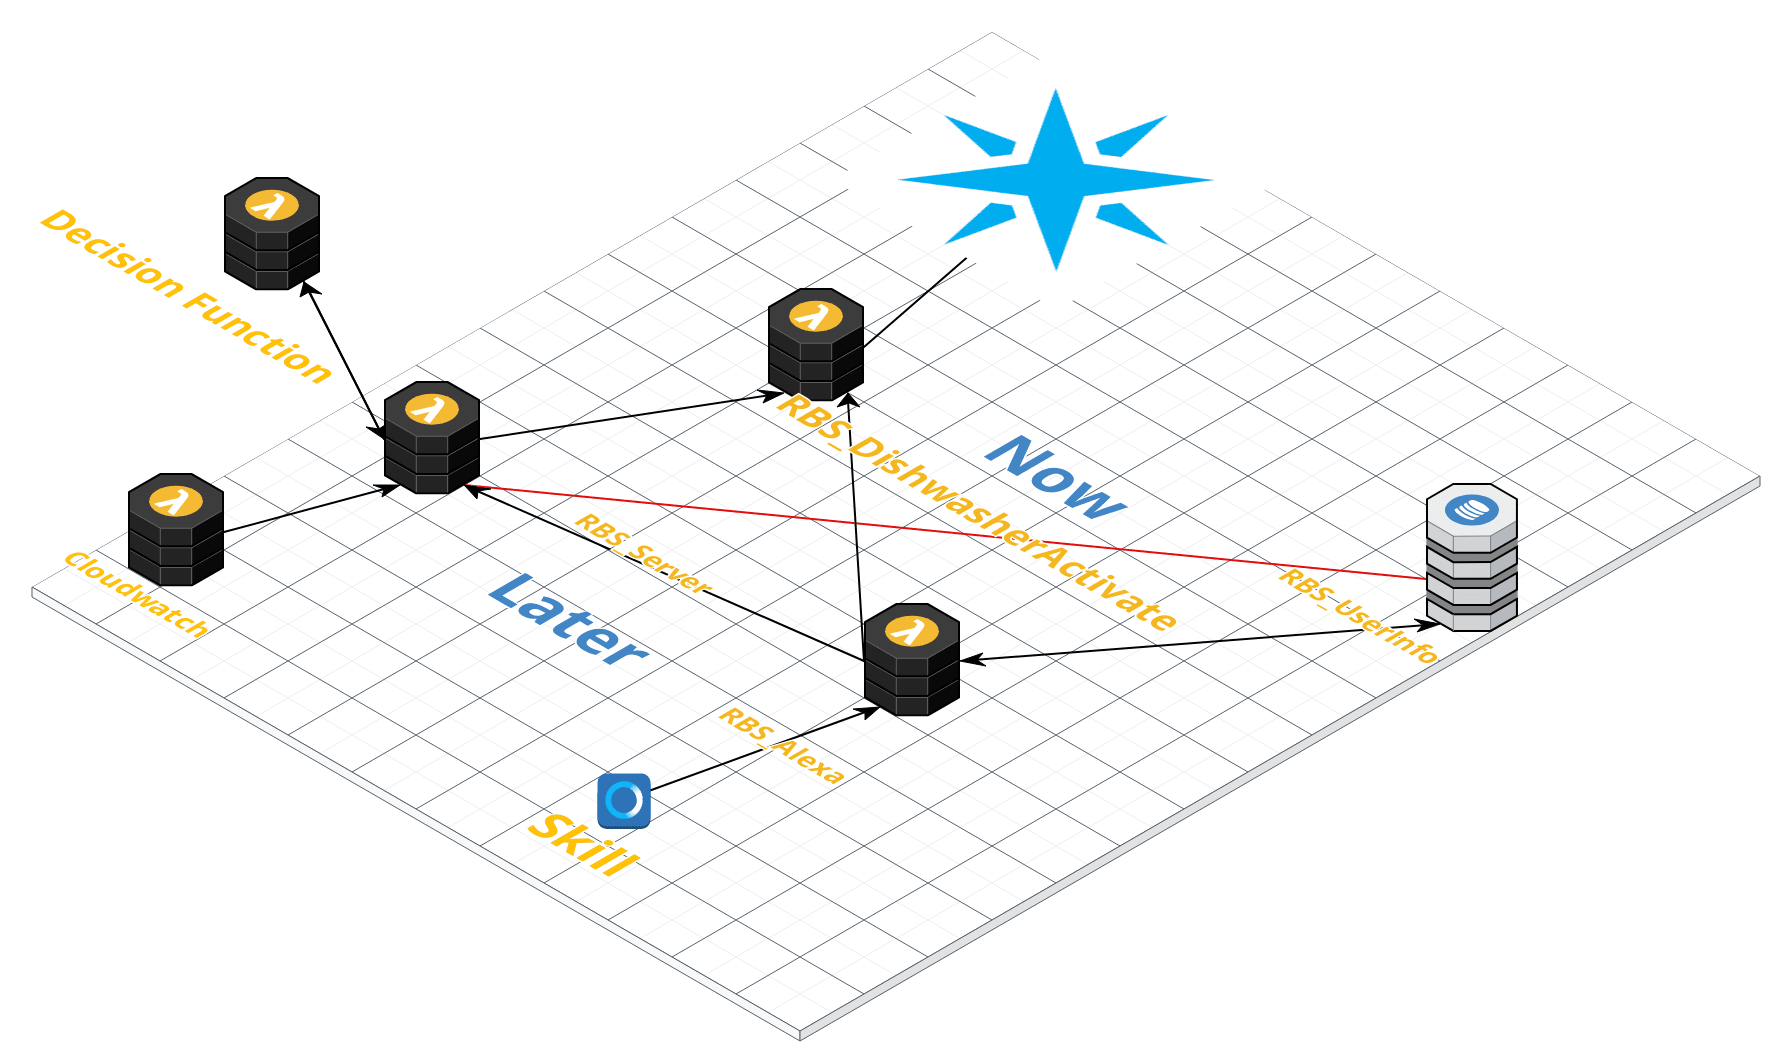
\includegraphics[width=\paperwidth,height=\paperheight,keepaspectratio]{pictures/architecture}
\end{frame}

\begin{frame}
    
\includegraphics[width=0.5\paperwidth,height=0.5\paperheight,keepaspectratio]{pictures/october}
    \begin{outline}
        \1<1-> First two weeks:
        \2<1-> Revived Old Infrastructure
        \1<1-> Second two weeks:
        \2<1-> Scaled the existing infrastructure to work with two appliances for one user
        when invoking the appliance immediately.
        \1<2-> Noticed problem in workflow.
    \end{outline}
\end{frame}

\begin{frame}
    \frametitle{Workflow Challenges}
    \begin{outline}
        \1<1-> By its very nature, serverless computing is a black box \cite{Baldini2017}:
        \2<2-> Inability to work locally:
        \3<3-> Limits version control.
        \3<4-> Limits teamwork.
        \3<5-> Limits programming tool usage (ie debuggers and editor customization)
        \2<6-> Inability to test:
        \3<7-> Introduces bugs into existing code.
        \3<8-> Leads to longer development time.
        \1<9-> Solution: Devops 
    \end{outline}
\end{frame}

\begin{frame}
    \frametitle{Devops Developments}
    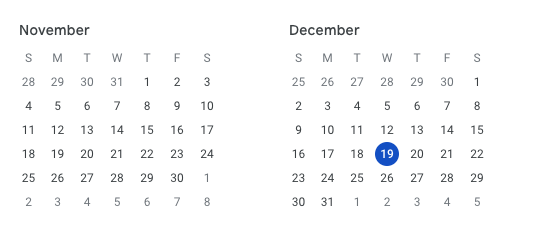
\includegraphics[width=0.5\paperwidth,height=0.5\paperheight,keepaspectratio]{pictures/nov_dec}
    \begin{outline}
        \1<1-> A script that allows for remote execution and uploading of lambda function code.
        \2<1-> First two weeks of November.
        \1<2-> Infrastructure as Code and learned common testing frameworks.
        \2<2-> Second two weeks of November.
        \1<3-> Testing frameworks and tests for Alexa Code and Lambda Function Code
        \2<3-> December
        \1<4-> Using these tools, I've made, thus far, a few slight changes.
    \end{outline}
\end{frame}

\begin{frame}
    \frametitle{Progress with Respect to Milestones}
    \begin{outline}
    \1 December 2018
    \2 Document half of the repository code. \textcolor{green}{25\%}
\2 \st{Devise a local workflow for the development of the Alexa UI.}
    \2 Refactor and test a function called \st{RBS\_Lambda} RBS\_dishwasher\_activate. \textcolor{green}{100\%}

    \2 Have a technical report of the prediction models tried by the group up until now. \textcolor{green}{0\%}
    \1 November 2018
    \2 Devise a local workflow for AWS lambda. At present, we use AWS's interface for most of our programming. We need a local workflow to
    streamline testing and development.\textcolor{green}{100\%}

\2 \st{Refactor and test a function called RBS\_argmin.}
    \2 Refactor and test a function called RBS\_server. \textcolor{green}{75\%}
    \2 Refactor and test a function called RBS\_Alexa \textcolor{green}{75\%}

    \end{outline}
\end{frame}

\begin{frame}
    \frametitle{Future Work}
    \begin{outline}
        \1 <1-> Devise a way of remotely 
        verifying whether the infrastructure caused the device to switch on at an ``optimal'' time.
        \1 <2-> Devise a way to simulate many clients using this service and to test the ability of the service to handle their requests.
        \1 <3-> Expand the range of utterances the Alexa front end can use.
        \1 <4-> Make the dialogues interactive.
        \1 <5-> Change the database schema to remove duplication of appliance information.
        \1 <6-> Refactor RBS\_server to use
        multiple devices.
    \end{outline}
\end{frame}

\begin{frame}[allowframebreaks]
  \frametitle<presentation>{Further Reading}    
  \begin{thebibliography}{10}    
  \beamertemplatearticlebibitems
  \bibitem{Jemand2000}
    S. Reed.
    \newblock Power prices go negative in germany, a positive for energy
users    
\newblock {\em New York Times}
  \beamertemplatearticlebibitems
  \bibitem{Baldini2017}
    Baldini
    \newblock Serverless computing: Current trends and open problems
\newblock {\em Research Advances in Cloud Computing}
  \beamertemplatearticlebibitems
  \bibitem{Lombard2008}
    Lombard
    \newblock A review on buildings energy consumption information.
\newblock {\em  Energy and Buildings}
  \beamertemplatearticlebibitems
  \bibitem{Faruqui2010}
  Faruqui
    \newblock The impact of informational feedback on energy consumption—A survey of the experimental evidence
\newblock {\em  Energy}
  \beamertemplatearticlebibitems
  \bibitem{Mooney2015}
  Mooney
    \newblock There’s a big change coming to how we power our homes — and it isn’t about solar or batteries
\newblock {\em Washington Post}
  \beamertemplatearticlebibitems
  \bibitem{Sowers2017}
  Sowers
    \newblock A smart power outlet for electric devices that can benefit from Real-Time Pricing
\newblock {\em 2017 International Conference on Control, Electronics, Renewable Energy and Communications (ICCREC)}
  \end{thebibliography}
\end{frame}

\end{document}

